\documentclass[10pt,twocolumn,a4paper]{article}
\usepackage[margin=18mm,columnsep=6mm]{geometry}
\usepackage[T1]{fontenc}
\usepackage{times}
\usepackage{graphicx,booktabs,amsmath,xcolor,float,tabularx,array}
\usepackage[font=small,labelfont=bf]{caption}
\usepackage{titlesec}
\usepackage[hidelinks]{hyperref}
\usepackage{listings}
\lstset{basicstyle=\ttfamily\footnotesize,columns=fullflexible,frame=single,framerule=0.3pt,
  keywordstyle=\color{blue!60!black}\bfseries,commentstyle=\color{gray},language=C++,
  xleftmargin=2pt,xrightmargin=2pt,aboveskip=4pt,belowskip=4pt}

\titleformat{\section}{\normalfont\large\bfseries}{\Roman{section}.}{0.5em}{\MakeUppercase}
\titleformat{\subsection}{\normalfont\normalsize\itshape}{\Alph{subsection}.}{0.5em}{}
\titlespacing*{\section}{0pt}{8pt}{4pt}
\titlespacing*{\subsection}{0pt}{6pt}{3pt}
\renewcommand{\thesection}{\Roman{section}}
\renewcommand{\thesubsection}{\thesection.\Alph{subsection}}

\title{\vspace{-6mm}\Large\bfseries Design and Verification of a Low-Cost Arduino-Based\\ Plant Growth Monitoring and Control System}
\author{Muhammad Ali Sadiq\\
\small M.Eng.\ Mechatronics \& Cyber-Physical Systems, Deggendorf Institute of Technology, Germany\\
\small \url{https://github.com/turtleshelp/automated-plant-monitoring}}
\date{\small November 2026}

\begin{document}
\maketitle

\begin{abstract}
\noindent This paper presents a low-cost embedded system that monitors and regulates the growing conditions of a single plant. An Arduino Uno reads light intensity, air temperature, relative humidity, soil moisture and the water level of a supply tank, and switches a grow lamp, fan, heat lamp, water spray and a relay-driven irrigation pump to keep each quantity inside an optimal band. All readings and actuator states are shown on a $20\times4$ character LCD and streamed over a serial link as CSV for logging. The system originated as a 2020 university course project and was redesigned in 2026: the control rules were separated into a hardware-independent module with two-threshold (hysteresis) logic, sensor faults are handled fail-safe, the main loop was made non-blocking, and a dry-run interlock was added for the pump. The design is verified at three levels: 27 host-side unit-test assertions on the decision logic, a full-circuit simulation in Wokwi, and hardware tests of the 2020 prototype. The source code, simulation and wiring diagram are openly available.
\end{abstract}

\noindent\textbf{Keywords:} embedded systems, Arduino, plant monitoring, automatic irrigation, hysteresis control, simulation-based verification

\section{Introduction}
Keeping a plant in good condition requires regular attention to light, temperature, humidity and soil moisture. Doing this by hand is time-consuming and inconsistent: watering is easily forgotten or overdone, and indoor light and climate change over the day. A small embedded controller can measure these quantities continuously and react automatically, which reduces manual work and avoids wasting water.

The goal of this work is a system that is cheap, built from widely available hobby components, and simple enough to verify thoroughly. The contributions are:
\begin{itemize}\setlength\itemsep{0pt}
\item a complete sensing-and-actuation design for five environmental quantities on a single 8-bit microcontroller;
\item a control layer written as a pure function with explicit hysteresis bands and fail-safe behaviour on sensor faults, so that it can be unit-tested on a PC;
\item a reproducible verification setup: unit tests plus a public full-circuit simulation that anyone can run in a web browser without hardware.
\end{itemize}

Section~\ref{sec:design} describes the hardware and control design, Section~\ref{sec:impl} the software implementation, Section~\ref{sec:verif} the verification results, and Section~\ref{sec:disc} limitations and future work.

\section{System Design}\label{sec:design}
\subsection{Architecture}
Fig.~\ref{fig:arch} shows the system architecture. Four sensor channels feed an Arduino Uno (ATmega328P, 16\,MHz, 10-bit ADC)~\cite{atmega,uno}. The firmware samples all inputs, evaluates the control rules and updates the outputs once every 2\,s. The outputs are six digital lines (five indicator/actuator channels and one relay), an I$^2$C LCD and a serial log.

\begin{figure*}[t]
\centering
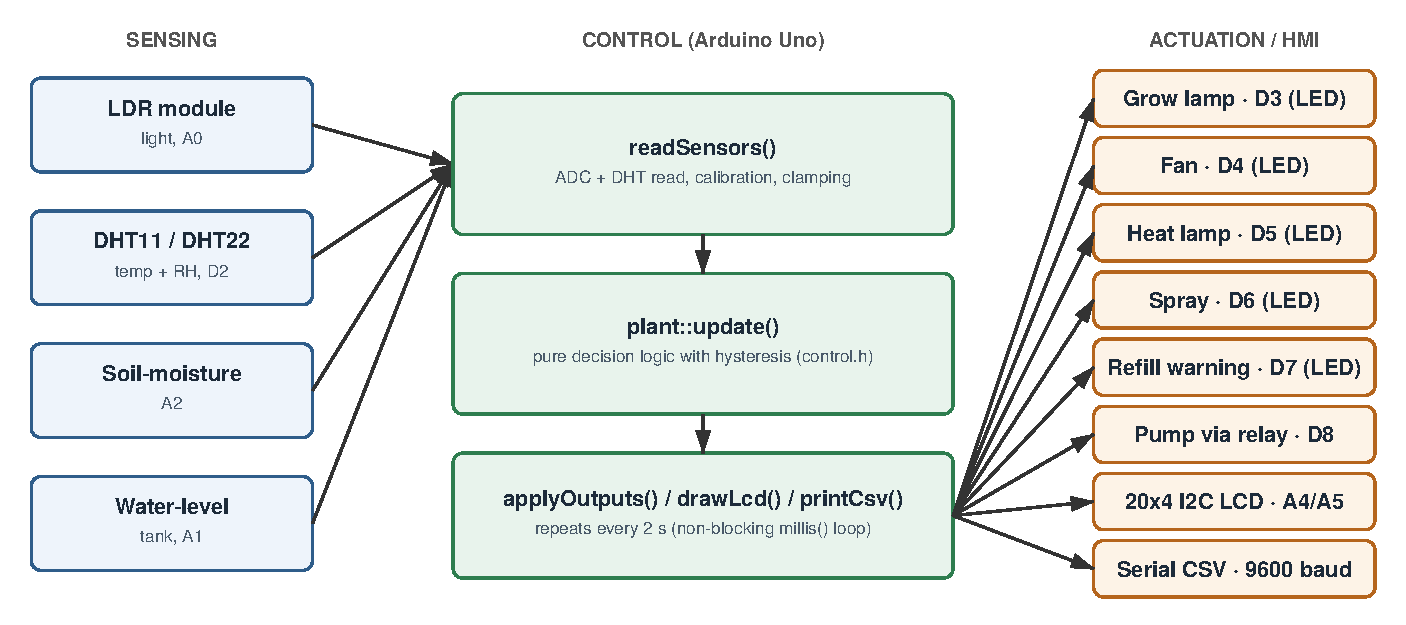
\includegraphics[width=0.82\textwidth]{fig/architecture.pdf}
\caption{System architecture. Each cycle reads all sensors, evaluates the pure decision function \texttt{plant::update()} and then drives the outputs, LCD and serial log.}
\label{fig:arch}
\end{figure*}

\subsection{Hardware}
\textbf{Sensors.} Temperature and relative humidity are measured by a DHT-family single-wire sensor: a DHT11 in the prototype and a DHT22 (AM2302) in the simulation~\cite{dht11,dht22}. Light is measured with a light-dependent resistor (LDR) module whose analogue output rises as the light level falls. Soil moisture and tank water level are measured with analogue probes; in the simulation both are represented by potentiometers.

\textbf{Outputs.} The grow lamp, fan, heat lamp, spray and the tank-refill warning are each represented by an LED with a 220\,$\Omega$ series resistor, which shows the switching decision without mains-powered loads. The irrigation pump is driven through a relay module on D8, so a real pump can be connected to the relay contacts with its own supply. A $20\times4$ HD44780-compatible LCD with an I$^2$C backpack (address 0x27) uses only the A4/A5 bus lines~\cite{hd44780}.

\textbf{Pin assignment.} Table~\ref{tab:pins} lists the pin map; the full wiring is shown in Fig.~\ref{fig:wiring}. Pins D0/D1 are deliberately left free so that the serial log does not conflict with any output.

\begin{table}[h]
\centering\small
\caption{Pin assignment (Arduino Uno)}\label{tab:pins}
\begin{tabular}{@{}ll@{}}
\toprule
Pin & Function \\ \midrule
D2 & DHT11/DHT22 data \\
A0 & LDR module (analogue) \\
A1 & Water-level sensor \\
A2 & Soil-moisture sensor \\
A4 / A5 & LCD I$^2$C SDA / SCL \\
D3--D7 & Grow lamp, fan, heat lamp, spray, refill warning \\
D8 & Relay module input (pump) \\
\bottomrule
\end{tabular}
\end{table}

\begin{figure*}[t]
\centering
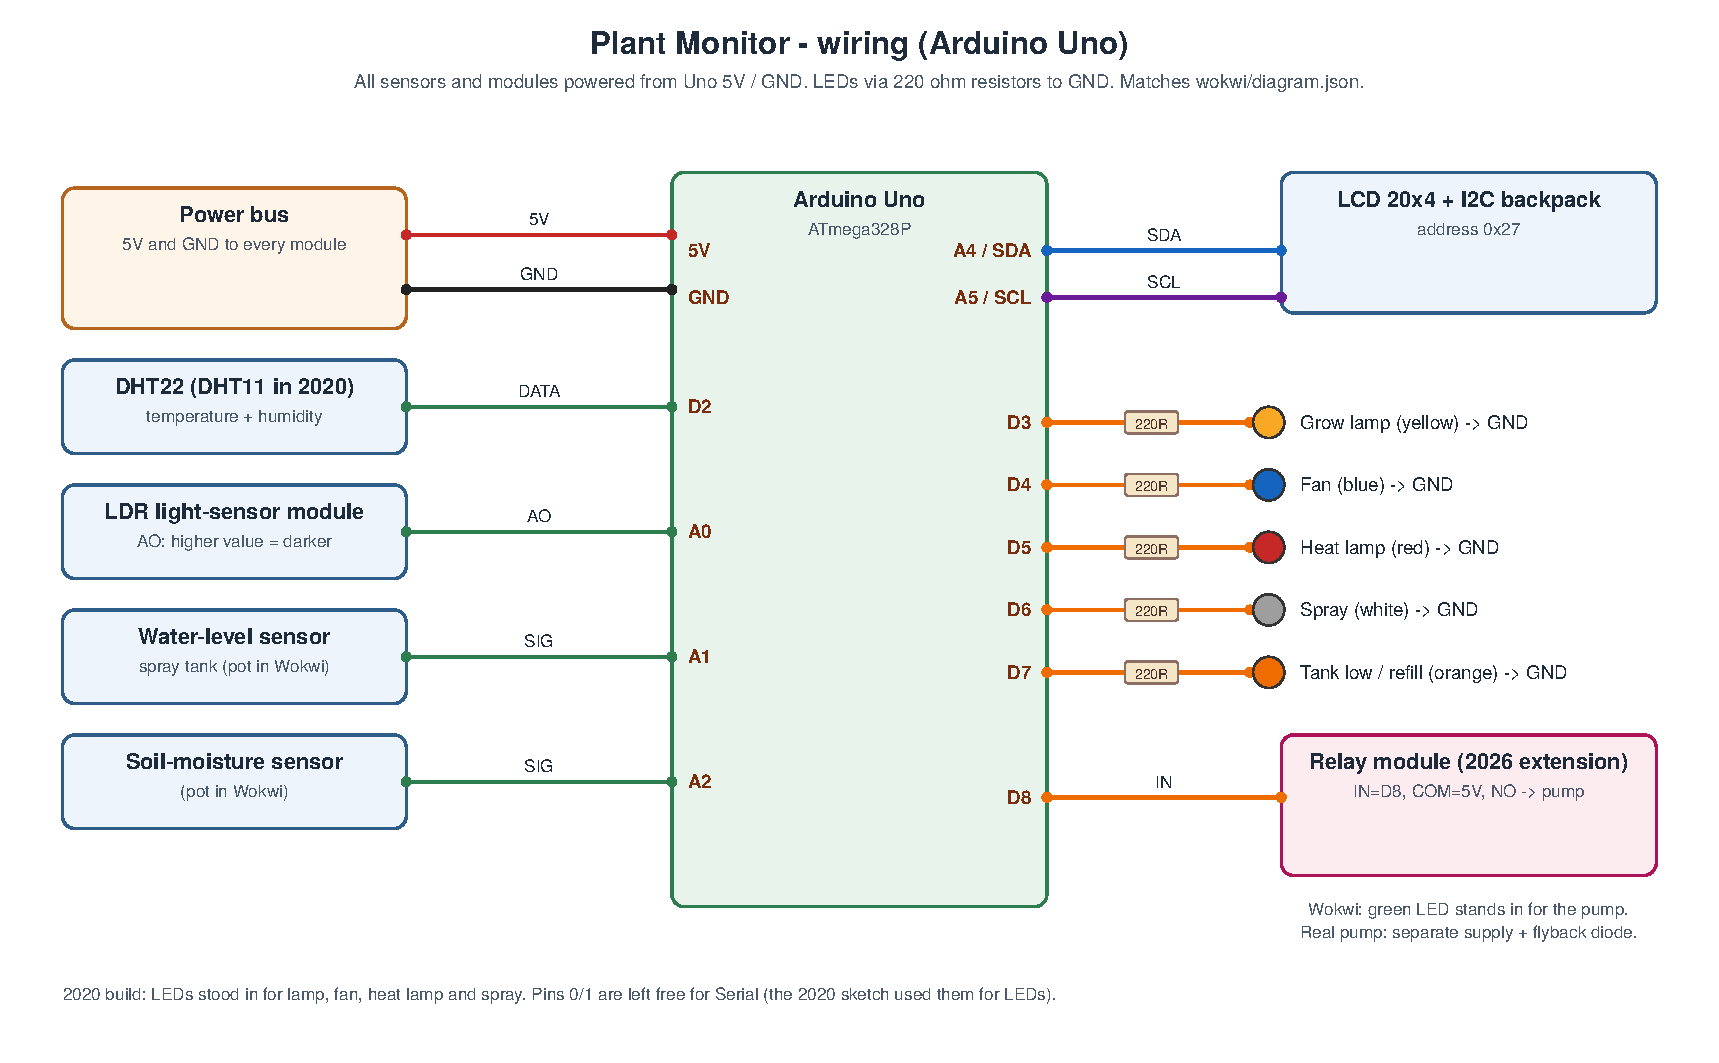
\includegraphics[width=0.86\textwidth]{fig/wiring.pdf}
\caption{Wiring diagram. All modules share the Uno's 5\,V and GND; each indicator LED has a 220\,$\Omega$ series resistor.}
\label{fig:wiring}
\end{figure*}

\subsection{Control Strategy}
Each quantity is controlled by a simple on/off rule with two thresholds (Table~\ref{tab:rules}). Between the two thresholds the output keeps its previous state. This hysteresis band prevents an actuator from toggling rapidly when a reading hovers around a single set point. The fan is shared: it runs if either the temperature or the humidity is too high.

Two safety rules take priority over the others:
\begin{itemize}\setlength\itemsep{0pt}
\item \emph{Dry-run interlock:} when the tank level falls below 20\,\% a refill warning is raised and the pump is forced off. The warning clears only above 30\,\%, so it does not flicker around the threshold.
\item \emph{Sensor fault:} if the DHT sensor returns no valid reading (NaN), the spray, fan and heat lamp are switched off rather than acting on stale data.
\end{itemize}

\begin{table}[h]
\centering\small
\caption{Control rules. Inside each band the output holds its last state.}\label{tab:rules}
\begin{tabular}{@{}lll@{}}
\toprule
Input & Condition & Action \\ \midrule
Light (raw ADC) & $>200$ (dark) & Grow lamp ON \\
 & $<150$ (bright) & Grow lamp OFF \\
Humidity & $>60$\,\% & Fan ON, spray OFF \\
 & $<50$\,\% & Spray ON \\
Temperature & $>29$\,$^\circ$C & Fan ON \\
 & $<27$\,$^\circ$C & Heat lamp ON \\
Soil moisture & $<20$\,\% & Pump ON \\
 & $>50$\,\% & Pump OFF \\
Tank level & $<20$\,\% & Refill warning, pump locked \\
 & $>30$\,\% & Warning cleared \\
\bottomrule
\end{tabular}
\end{table}

\section{Software Implementation}\label{sec:impl}
\subsection{Structure}
The firmware is split into two files. \texttt{control.h} contains the thresholds, the \texttt{Readings} and \texttt{Outputs} data types and the decision function. It has no Arduino dependencies, so the same code is compiled for the ATmega328P and for a PC test harness. \texttt{plant\_monitor.ino} contains only the hardware layer: sensor reading, output writing, LCD formatting and the serial log.

The decision function is pure: its result depends only on the current readings and the previous output state.
\begin{lstlisting}
Outputs update(const Readings& r,
               const Outputs& prev);
\end{lstlisting}
This makes every rule, including the hysteresis behaviour, testable with simple input sequences.

\subsection{Sensor Conditioning}
Analogue readings are converted to percentages by a linear two-point mapping that also works for inverted sensors (where a higher ADC value means drier soil) and is clamped to 0--100\,\%. The clamp fixes a defect of the 2020 prototype, whose unclamped mapping produced physically impossible values such as $-86$\,\% moisture when the probe read outside its calibrated range (Section~\ref{sec:proto}).

\subsection{Timing and User Interface}
The main loop is non-blocking and scheduled with \texttt{millis()}. Sensors are sampled every 2\,s, which respects the minimum sampling interval of the DHT sensors~\cite{dht22}. The prototype instead used a fixed \texttt{delay(2000)} per display screen, so one full update took several seconds and the controller could not react in between. The upper two LCD rows always show the five readings; the lower two rows alternate every 3\,s between the lamp/fan/heat/spray states and the pump/tank states. Each LCD row is written as exactly 20 characters, which overwrites old text without clearing the display and avoids flicker. Every sample is also printed as one CSV line (readings followed by the six output states) at 9600\,baud.

\section{Verification and Results}\label{sec:verif}
\subsection{Unit Tests}
The decision logic was tested on a PC (g++ 13, C++11) with 27 assertions covering: the clamped percentage mapping, including the out-of-range case that produced $-86$\,\% in the prototype; each threshold and its hold-in-band behaviour; the fan being driven by temperature \emph{or} humidity; fail-safe shutdown on a DHT fault; pump hysteresis; and the tank-level interlock with its 20/30\,\% hysteresis. All assertions pass. The firmware itself was additionally compiled on the host against stub Arduino headers to check it for syntax and type errors.

\subsection{Full-Circuit Simulation}
The complete circuit of Fig.~\ref{fig:wiring} was built in Wokwi, a browser-based simulator for the AVR microcontroller and its peripherals~\cite{wokwi}, using the same firmware and the Adafruit DHT and LiquidCrystal\_I2C libraries~\cite{adafruitdht,lcdi2c}. Table~\ref{tab:sim} lists two test cases with the readings and output states taken from the simulated serial log. Both match the rules in Table~\ref{tab:rules}: with an empty tank, the refill warning is raised and the pump is held off even though the soil reads 100\,\% wet; with dry soil and a 68\,\% full tank, the relay is energised and the pump runs. Fig.~\ref{fig:sim} shows the second case: the LCD, the indicator LEDs, the energised relay and the pump LED all match the logged state.

\begin{table}[h]
\centering\small\setlength{\tabcolsep}{4pt}
\caption{Simulation test cases (from the Wokwi serial log). L = light (raw ADC), T = temperature, H = humidity, S = soil, W = tank.}\label{tab:sim}
\begin{tabular}{@{}lcc@{}}
\toprule
 & Case 1 & Case 2 \\ \midrule
L / T / H & 250 / 24.0\,$^\circ$C / 40\,\% & 250 / 24.0\,$^\circ$C / 40\,\% \\
S / W & 100\,\% / 0\,\% & 5\,\% / 68\,\% \\ \midrule
Grow lamp & ON & ON \\
Fan & OFF & OFF \\
Heat lamp & ON & ON \\
Spray & ON & ON \\
Pump & \textbf{OFF} (locked) & \textbf{ON} \\
Refill warning & \textbf{ON} & OFF \\
\bottomrule
\end{tabular}
\end{table}

\begin{figure}[t]
\centering
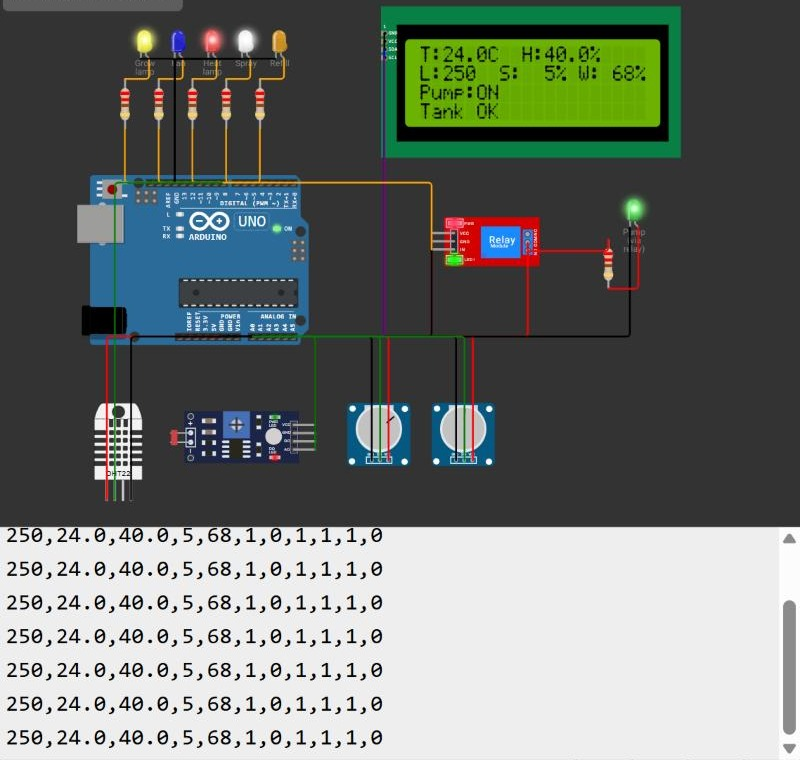
\includegraphics[width=\columnwidth]{fig/wokwi-simulation.jpg}
\caption{Wokwi simulation of the full circuit (test case 2). The LCD shows the readings and pump state, the relay is energised and the green pump LED is lit; the serial log is at the bottom.}
\label{fig:sim}
\end{figure}

The simulation is public and runs in a web browser without any hardware: \url{https://wokwi.com/projects/480434156220494849}. Clicking the DHT22, the LDR module or either potentiometer during a run changes the corresponding reading, so each rule in Table~\ref{tab:rules} can be checked interactively.

\subsection{2020 Hardware Prototype}\label{sec:proto}
The 2020 prototype was built on an Arduino Uno with a DHT11, an LDR, analogue soil-moisture and water-level probes, a $20\times4$ I$^2$C LCD and indicator LEDs, and was tested on the bench. Fig.~\ref{fig:proto} shows three LCD states recorded during these tests: high humidity (73\,\%) switching the fan on, low light (raw ADC 295) switching the lamp on, and an empty tank being reported as low.

\begin{figure}[t]
\centering
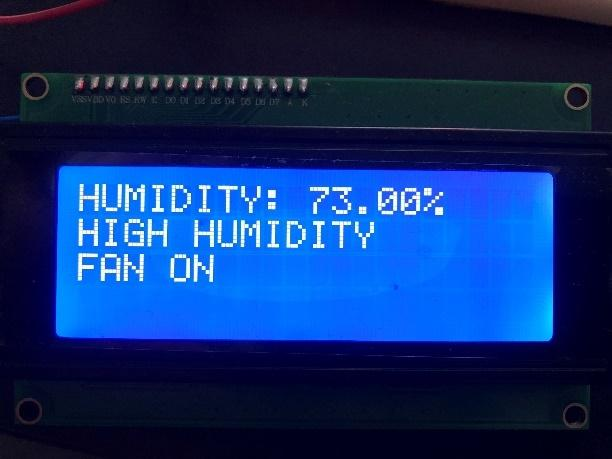
\includegraphics[width=0.32\columnwidth]{fig/2020-hardware-lcd-humidity.jpg}\hfill
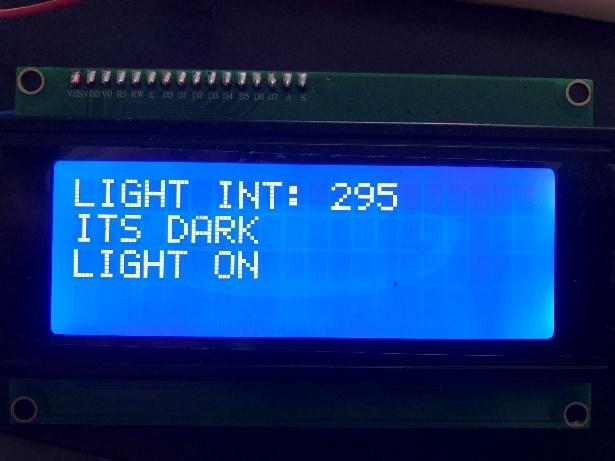
\includegraphics[width=0.32\columnwidth]{fig/2020-hardware-lcd-light.jpg}\hfill
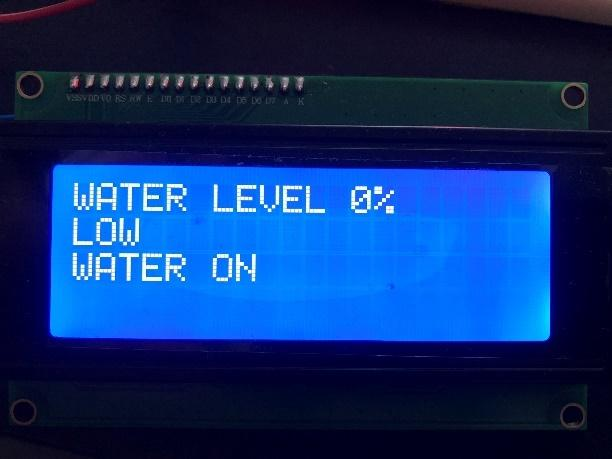
\includegraphics[width=0.32\columnwidth]{fig/2020-hardware-lcd-water-level.jpg}
\caption{2020 prototype on hardware: high humidity $\rightarrow$ fan on (left), dark $\rightarrow$ light on (centre), tank level 0\,\% (right).}
\label{fig:proto}
\end{figure}

Readings were streamed over serial into a spreadsheet logger (Fig.~\ref{fig:log}). Over 15 samples spanning 31\,s at room conditions, the readings were stable: light 276--280, temperature 28.1--28.2\,$^\circ$C and humidity 76--77\,\%. The moisture channel, however, read $-85$ to $-86$\,\%. This is consistent with the prototype's unclamped mapping \texttt{map(raw, 550, 10, 0, 100)}: a raw reading near the top of the ADC range, as from a dry or disconnected probe, gives about $-86$\,\%. The 2026 design clamps the result (Section~\ref{sec:impl}) and covers this case with a unit test.

\begin{figure}[t]
\centering
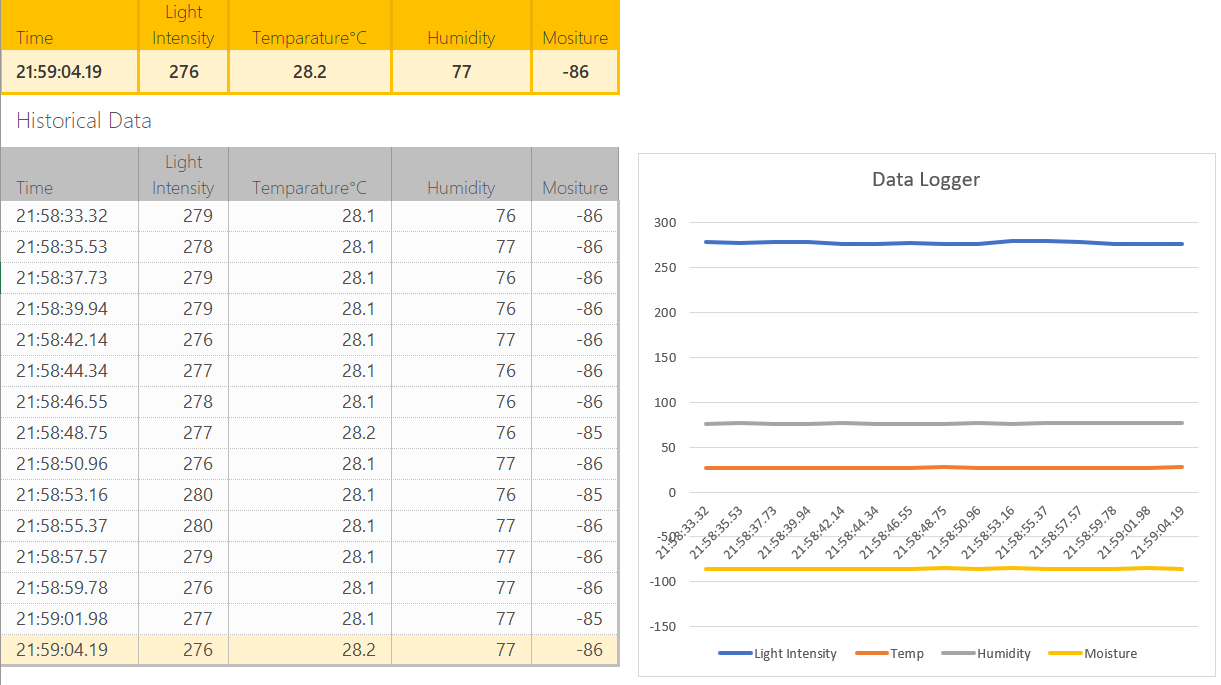
\includegraphics[width=\columnwidth]{fig/2020-data-log.png}
\caption{Serial data log of the 2020 prototype. The negative moisture values reveal the unclamped-mapping defect fixed in the 2026 design.}
\label{fig:log}
\end{figure}

A review of the prototype firmware found further defects that the redesign removes: range checks written as \texttt{150 > x < 200}, which C evaluates as \texttt{(150 > x) < 200} and is therefore always true; indicator LEDs on D0/D1, which conflict with the serial port; and re-initialisation of the LCD on every loop iteration.

\section{Discussion and Limitations}\label{sec:disc}
The 2026 design has been verified in simulation and by unit tests only; it has not been rebuilt on hardware. The lamp, fan, heat lamp and spray are represented by LEDs, and no real pump has been driven. The soil and tank calibration constants come from the prototype and have not been re-measured. The thresholds are fixed values chosen for a generic indoor plant; they are not tuned to a particular species. On/off control with hysteresis is appropriate for these slow processes, but watering until the probe reads ``wet'' can overshoot because water takes time to soak through the soil.

\section{Conclusion and Future Work}
A low-cost plant monitoring and control system was designed around an Arduino Uno and five sensed quantities, with a hardware-independent decision layer, hysteresis on every actuator, fail-safe handling of sensor faults and a dry-run interlock for the pump. Unit tests, a public full-circuit simulation and prototype hardware tests show that the control rules behave as specified, and the redesign removes the defects found in the prototype. Future work includes: PWM dimming of the grow lamp instead of on/off switching; capacitive soil probes with a two-point calibration routine; pulsed watering with a soak delay; wireless logging and alerts, for example on an ESP32; and a hardware rebuild with real actuators to validate the simulation results.

\begin{thebibliography}{9}\small\setlength\itemsep{1pt}
\bibitem{atmega} Microchip Technology, \emph{ATmega328P Datasheet}. [Online]. Available: \url{https://www.microchip.com/en-us/product/ATmega328P}
\bibitem{uno} Arduino, \emph{Arduino UNO R3 Documentation}. [Online]. Available: \url{https://docs.arduino.cc/hardware/uno-rev3}
\bibitem{dht11} Aosong Electronics, \emph{DHT11 Humidity \& Temperature Sensor Datasheet}.
\bibitem{dht22} Aosong Electronics, \emph{AM2302 (DHT22) Digital-Output Relative Humidity \& Temperature Sensor Datasheet}.
\bibitem{hd44780} Hitachi, \emph{HD44780U (LCD-II) Dot Matrix Liquid Crystal Display Controller/Driver Datasheet}.
\bibitem{wokwi} Wokwi, \emph{Wokwi Online Electronics Simulator}. [Online]. Available: \url{https://wokwi.com}
\bibitem{adafruitdht} Adafruit Industries, \emph{DHT Sensor Library}. [Online]. Available: \url{https://github.com/adafruit/DHT-sensor-library}
\bibitem{lcdi2c} F.~de~Brabander \emph{et al.}, \emph{LiquidCrystal\_I2C Library}. [Online]. Available: \url{https://github.com/johnrickman/LiquidCrystal_I2C}
\end{thebibliography}

\end{document}
